\documentclass{article}
\usepackage[utf8]{inputenc}
\usepackage{graphicx}
\usepackage[left=2cm,right=2cm,top=3cm,bottom=3cm]{geometry}
\title{MCS: Compte-rendu}

\begin{document}
\maketitle
\section{Matrice de confusion}
	\begin{figure}[h]
		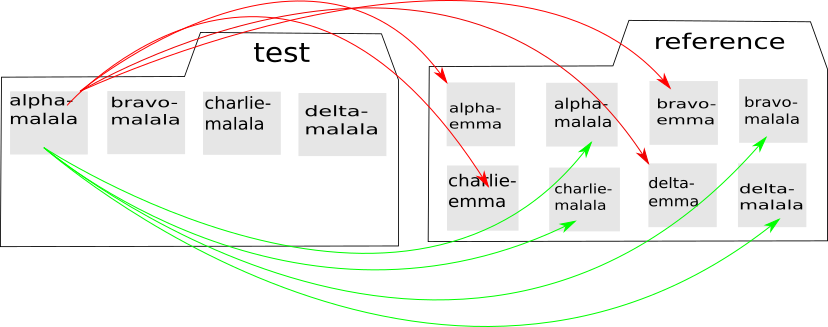
\includegraphics[scale=0.5]{compte-rendu.png}
	\end{figure}
\section{Résultats et analyse}
	\subsection{Test 1: Exemple simple sur enregistrement perso}
	\begin{table}[h]
		\begin{tabular}{|c|c|c|c|c|}
			\hline
			& alpha emma, malala & bravo emma, malala & charlie emma, malala & delta emma, malala\\
			\hline
			alpha-malala & 2 & 0 & 0 & 0 \\
			\hline
			bravo-malala & 1 & 1 & 0 & 0 \\
			\hline
			charlie-malala & 1 & 0 & 1 & 0 \\
			\hline
			delta-malala & 1 & 0 & 0 & 1 \\
			\hline
		\end{tabular}
	\end{table}
	\[
   	taux\ de\ reconnaissance = 62.5 \%
	\].
	\begin{itemize}
		\item Dans cet exemple, on a des 1 sur la diagonale car les distances entre les sons \textit{x-malala} sont égales à 0.\\
		\item Les 1 sur la première colonne signifie que les sons \textit{x-malala} comparés aux sons \textit{x-emma} se rapporchent le plus de \textit{alpha-emma}.
	\end{itemize}

	\subsection{Test 2: Exemple sur plus grande base de test}
		\subsubsection{Test 2.1: Corpus}
			//TODO
		\subsubsection{Test 2.2: Enregistrements personnels}
			//TODO
\end{document}

